% CVPR 2027 review submission
\documentclass[10pt,twocolumn,letterpaper]{article}
\usepackage[review]{cvpr}
\def\confName{CVPR}
\def\confYear{2027}
\definecolor{cvprblue}{rgb}{0.21,0.49,0.74}
\usepackage[pagebackref,breaklinks,colorlinks,allcolors=cvprblue]{hyperref}
\usepackage{microtype}

\title{Reliable Strictly Local Floorplan Editing\\under Imperfect Controls}
\author{Anonymous CVPR submission}
\date{}

\begin{document}
\maketitle

\begin{abstract}
Floorplan editors often report edit accuracy without establishing that unrelated
architecture remains unchanged. We study a complementary requirement: reliable
local execution under an explicit control interface. A request consists of an
old CAD state, a declared edit region, and a typed control change. The output may
change only inside the declared region and must remain structurally legal. We
evaluate this contract in two regimes. Under target-derived oracle controls,
FloorFlow reaches Delta-IoU 0.956703--0.999801 and Delta-MSE
0.000019--0.000096 across five operations while preserving outside pixel, room,
polygon, wall, opening, and unaffected-edge content exactly. Under target-free
predicted controls, it preserves the same outside contract, produces structurally
plausible plans over five repeated validation seeds, and abstains from every
unsupported or ambiguous request in a development-exposed prompt audit. We keep
these safety properties separate from reference fidelity: predicted Room macro
IoU is 0.269701, raw watertightness is 0.816701, and an older-model semantic
diagnostic ranges from 0.00 to 0.92. The contribution is a scoped, auditable
editing result and a reproducible boundary between locality, legality, and
semantic realization, not a claim of complete benchmark superiority.
\end{abstract}

\section{Introduction}
A floorplan edit is not merely a plausible new drawing. It is a controlled
transition from an existing plan: the requested operation must be realized, the
unaffected architecture must remain untouched, and the result must remain legal.
These requirements are usually conflated in end-to-end metrics. A global
regeneration can score well on an image or vector comparison while silently
moving walls outside the requested region. Conversely, a perfectly local change
can preserve geometry while failing to perform the requested semantic operation.

We treat locality, topology legality, edit support, and semantic realization as
separate measurement axes. The input is an old plan, its control state, a
declared edit region, and a typed operation. FloorFlow composes a control change
only inside the declared domain, restores the outside layers exactly, and audits
the resulting topology. Unsupported wall movement, ambiguous global scope, and
conflicting instructions are routed to abstention rather than forced through the
generator.

The evaluation deliberately separates two evidence regimes. Oracle controls use
target-derived after-edit controls and establish an editing upper bound; they are
not deployable. Predicted controls are target-free at inference and expose the
real operating point, including weak reference fidelity and mixed semantic
success. A matched reconstruction wrapper, an outside-frozen editing-aware
control, deterministic composition-policy arms, and protocol attacks test whether
the observed locality and edit support can be explained by freezing alone.

Our contributions are:
\begin{itemize}
\item a strictly local typed-edit protocol with an explicit outside domain and
zero-tolerance preservation audit;
\item a scoped oracle-control anchor over 2,479 edits, five operations, and five
repeated execution seeds;
\item a target-free reliability audit that separates execution safety,
structural plausibility, raw topology, and reference fidelity;
\item matched controls and a deterministic composition ablation showing where the
measured gain comes from and where it does not;
\item a reproducible evidence release whose numerical claims are bound to a
source registry, frozen file identities, and case-level figure provenance.
\end{itemize}

The paper does not claim complete HouseMind or RPLAN superiority, full-CAD SOTA,
deployable free-text editing, or fresh held-out generalization. Those boundaries
are part of the result.

\section{Related Work}
HouseMind unifies floorplan understanding, generation, and editing with discrete
room-instance representations and reports edit and graph metrics on an RPLAN
natural-language protocol~\cite{housemind}. We use its published Delta-IoU and
Delta-MSE values only as cross-dataset context. The public table does not expose
strict outside preservation, locality violations, negative controls, or attack
sensitivity, so it cannot certify the contract studied here.

Raster2Seq reconstructs vector plans from raster inputs~\cite{raster2seq}. We use
an outside-frozen raster-to-vector redraw as a matched reconstruction wrapper.
This is a strong diagnostic against the concern that a locality wrapper alone
produces the reported result, but it is not a native editing model and we do not
attribute editing awareness to it. CE2EPlan studies boundary-conditioned vector
generation~\cite{ce2eplan}; generation evidence is not interpreted as editing
evidence.

Floorplan recognition and vectorization provide the geometric substrate.
CubiCasa5K supplies heterogeneous annotated plans~\cite{cubicasa}, while graph
representations such as GSDiff inform structured evaluation~\cite{gsdiff}. We do
not pool aligned, canonical-instance, and typed graph protocols, and we report
graph values as diagnostics rather than a ranking.

\section{Problem and Protocol}
\subsection{Control Transition}
Let $x_0$ be the old visible plan and $c_0$ its control state. A request contains
a normalized or control-grid edit region $R$ and a typed operation $a$. The
edited control is $c_1=T_a(c_0)$, and the model outputs
\begin{equation}
x_1=f(x_0,c_1,R).
\end{equation}
The old control state is an allowed input because engineering edits are applied
relative to an existing drawing and its constraints. The contract therefore asks
two separate questions: is the request supported, and does the output realize the
requested change without changing the rest of the plan?

\subsection{Strict Outside Domain}
The valid outside domain is
\begin{equation}
O = P \land \neg R \land \neg D_1(W_0 \lor W_1),
\end{equation}
where $P$ is the footprint, $W_0,W_1$ are pre- and post-edit wall support, and
$D_1$ is one-pixel dilation. Pixel, room-label, room-mask, polygon, wall, opening,
and unaffected-edge content outside $O$ is compared exactly. A change there is a
contract failure, not a small quality loss. The changed-control mask is an anchor
for the requested edit and cannot expand the allowed domain.

\subsection{Operations and Abstention}
The supported operations are room-type change, room addition, room removal,
opening deletion, and furniture deletion. Unsupported wall movement, ambiguous
global scope, and conflicting instructions trigger safe abstention. Abstention
returns the pre-edit plan and is never counted as a semantic edit.

\section{FloorFlow}
\subsection{Typed Control Routing}
FloorFlow represents rooms, walls, openings, furniture, and support regions as
typed control families. A typed router selects the family and spatial support
affected by the request. The routing policy used in the main evidence is
deterministic and adds no learned parameters over the matched no-graph arm. It is
therefore evaluated as a composition policy, not as a separately trained network.

\subsection{Local Composition}
The old plan, the predicted post-edit completion, and the edit support are
composed through a control-change gate. The gate admits the requested delta only
inside the declared region, then restores outside layers exactly. This operation
is intentionally conservative: it can preserve an unsupported local change when
the semantic execution is weak, but it cannot hide an outside violation behind a
small average error.

\subsection{Verification}
FP-Eval checks mandatory validity and conditional watertightness. FEVP checks the
five-layer outside contract and protocol attacks. Structural diagnostics report
wall continuity, opening alignment, furniture containment, outside-footprint
leakage, room overlap, and graph readouts. Raw watertightness and functional or
componentwise watertightness are always reported separately.

\begin{figure*}[t]
\centering
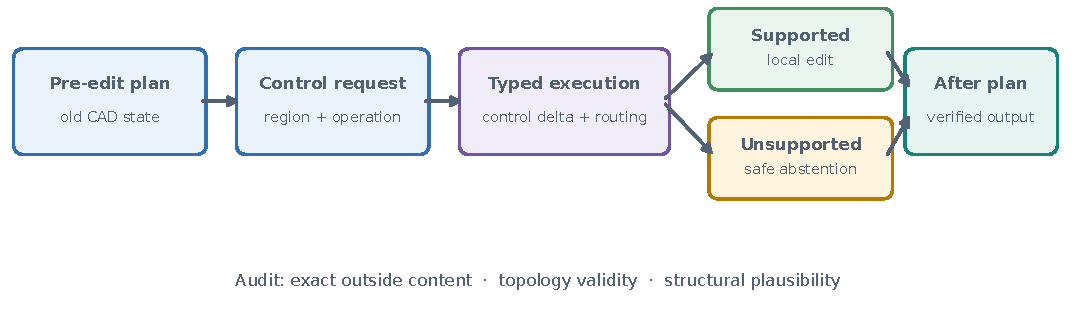
\includegraphics[width=0.96\textwidth]{figures/floorplan_protocol_overview_v1.pdf}
\caption{Strict local editing as a typed control transition. Supported requests
are executed and audited; unsupported or ambiguous requests return a safe
abstention. The outside contract is checked independently of edit fidelity.}
\label{fig:protocol}
\end{figure*}

\section{Experimental Design}
\subsection{Populations and Exposure}
Oracle-control results use CubiCasa5K test503 with 2,479 eligible edits across
five operations and five repeated execution seeds. The primary local-delta path
is deterministic on fixed rows; repeated seeds verify reproducibility rather than
create independent floorplans.

Predicted structural reasonableness uses val491 with 491 target-free cases per
seed and five repeated seeds. The operation audit contains 738 prompts from a
development-exposed test manifest. Its row metadata declares \texttt{split=test};
legacy summary fields claiming val191 are ignored. A separate semantic diagnostic
uses an older val191 model and is never pooled with the selected release model or
with oracle rows.

Fresh held-out generalization is marked
\texttt{optional\_generalization\_not\_evaluated}. A new held-out claim would
require a separate pre-access freeze, one execution, and retention of every
negative result. It is not a prerequisite for the scoped claims in this paper.

\subsection{Statistical Units}
Delta-IoU intervals resample floorplans with replacement and average all edit
instances inside a sampled floorplan. Repeated seed rows are not treated as
independent plans. Paired baselines use one difference per unique floorplan and
Holm adjustment across five operations. The seed19 trace audit recomputes all
2,479 oracle rows with zero IoU error; other seeds remain reported reproducibility
checks.

\subsection{Matched Controls}
The reconstruction wrapper applies Raster2Seq inside an outside-frozen local
redraw. The editing-aware control consumes the same declared pre/post controls but
recomputes its own paired FloorFlow row. Deterministic composition arms remove
typed routing, dense cross-attention, edit gating, or the structural graph while
keeping the measured rows fixed. The budget audit is post hoc and does not support
an efficiency claim.

\section{Results}
\subsection{Oracle-Control Editing Anchor}
Table~\ref{tab:oracle} reports the scoped oracle anchor. Room type, room addition,
and room removal exceed 0.999 Delta-IoU, while opening deletion and furniture
deletion reach 0.956703 and 0.987812. Outside exactness and FP-Eval validity are
1.0 for every operation. Pooled conditional watertightness is
0.957875--0.967491, and independent FEVP five-check validity ranges from 0.9124
to 0.9569.

These values measure binary change support. They do not prove requested-class
correctness: a visually large change can have high Delta-IoU while realizing the
wrong class. That boundary is why the paper reports semantic diagnostics
separately rather than interpreting the oracle metric as deployable accuracy.

\begin{table*}[t]
\centering
\caption{Oracle-control editing anchor on CubiCasa5K test503. Intervals resample floorplans; repeated seeds are not independent plans. Delta metrics measure change support, not target-class correctness.}
\label{tab:oracle}
\small
\begin{tabular}{lrrrrr}
\toprule
Operation & $N$ & $\Delta$IoU [95\% CI] & $\Delta$MSE & Outside exact & Vector validity \\
\midrule
Room type & 487 & 0.999199 [0.998420, 0.999747] & 0.000069 & 1.000000 & 0.956879 \\
Room add & 495 & 0.999801 [0.999545, 0.999990] & 0.000030 & 1.000000 & 0.955556 \\
Room remove & 500 & 0.999756 [0.999479, 0.999966] & 0.000019 & 1.000000 & 0.954000 \\
Opening delete & 502 & 0.956703 [0.941316, 0.970424] & 0.000096 & 1.000000 & 0.912351 \\
Furniture delete & 495 & 0.987812 [0.982565, 0.992375] & 0.000083 & 1.000000 & 0.951515 \\
\bottomrule
\end{tabular}
\par\smallskip\footnotesize Pooled FP-Eval validity 1.000; conditional watertightness 0.9579--0.9675. FEVP five-check validity 0.9124--0.9569.
\end{table*}


\begin{table*}[t]
\centering
\caption{Same-case matched controls and deterministic composition-policy ablation. Raster2Seq is an outside-frozen wrapper and the editing-aware control is intentionally weak. The budget audit is post hoc and does not claim efficiency.}
\label{tab:matched}
\small
\begin{tabular}{lrrrrrr}
\toprule
Operation & $N$ & FloorFlow & Raster2Seq & Editing-aware & Gain vs R2S & Gain vs editing \\
\midrule
Room type & 487 & 0.999199 & 0.137160 & 0.909800 & 0.862039 & 0.089486 \\
Room add & 495 & 0.999801 & 0.166756 & 0.995985 & 0.833044 & 0.004015 \\
Room remove & 500 & 0.999756 & 0.177266 & 0.998508 & 0.822490 & 0.001340 \\
Opening delete & 502 & 0.956703 & 0.189491 & 0.731151 & 0.767212 & 0.225552 \\
Furniture delete & 495 & 0.987812 & 0.145367 & 0.742469 & 0.842445 & 0.245343 \\
\bottomrule
\end{tabular}
\par\medskip
\begin{tabular}{lrrrrrrr}
\toprule
Arm & Outside px & Outside room & Violation & $\Delta$IoU & Node F1 & Edge F1 & GED \\
\midrule
Typed routing & 1.000000 & 1.000000 & 0.000000 & 0.937473 & 0.955068 & 0.890007 & 2.120855 \\
Dense routing & 0.999545 & 0.999470 & 0.000455 & 0.887741 & 0.953797 & 0.887080 & 2.185478 \\
No edit gating & 0.986115 & 0.983599 & 0.013885 & 0.853715 & 0.949057 & 0.874121 & 2.448649 \\
No structural graph & 1.000000 & 1.000000 & 0.000000 & 0.888817 & 0.953819 & 0.887200 & 2.182251 \\
\bottomrule
\end{tabular}
\par\smallskip\footnotesize Typed routing: $\Delta$IoU gain +0.048656 and GED change -0.061396 at matched routing budget, with 3.1925 vs 0.2666 ms mean routing latency. Efficiency is not claimed.
\end{table*}


\subsection{Target-Free Predicted Reliability}
Table~\ref{tab:predicted} separates structural plausibility from safety and
semantics. Across val491, raster plausibility is 0.984929, plan plausibility
0.986558, FP-Eval validity 1.0, functional watertightness 0.997963, and wall
continuity 0.995427. Room-face retention is 0.995655. Outside-footprint leakage
and room overlap are zero.

Raw watertightness is 0.816701, not 1.0. Of 491 footprints, 401 are
single-component and pass both raw and componentwise checks; 90 are
multi-component and exceed the standard single-region FP-Eval boundary. The
component-aware diagnostic does not redefine the raw metric. Predicted Room macro
IoU is only 0.269701, confirming that structural reasonableness is not reference
fidelity.

All 438 supported development-exposed prompts execute, all 300 unsupported or
ambiguous prompts abstain, and every row preserves outside pixel and room-label
content exactly with validity 1.0. This is a safety result. The older val191
semantic diagnostic remains mixed: room addition 92/100, room type 55/100, room
removal 20/100, opening deletion 30/59, and furniture deletion 0/15. Object-delete
and ghost-state contracts are separate execution checks and are not semantic
successes.

\begin{table*}[t]
\centering
\caption{Target-free predicted-control evidence. (A) Structural reasonableness on val491 across five repeated seeds. (B) Development-exposed safety prompts and a separately labeled older-model semantic diagnostic. Raw and functional watertightness are distinct.}
\label{tab:predicted}
\small
\begin{minipage}[t]{0.52\linewidth}
\centering
\begin{tabular}{lr}
\toprule
Metric & Mean \\
\midrule
Raster plausible & 0.984929 \\
Plan plausible & 0.986558 \\
Room coverage & 1.000000 \\
Room-face retention & 0.995655 \\
FP-Eval validity & 1.000000 \\
Raw watertight & 0.816701 \\
Functional watertight & 0.997963 \\
Wall continuity & 0.995427 \\
Opening-wall align & 0.993530 \\
Furniture containment & 1.000000 \\
Outside-footprint fraction & 0.000000 \\
Room overlap ratio & 0.000000 \\
Room macro IoU (diag.) & 0.269701 \\
\bottomrule
\end{tabular}
\end{minipage}\hfill
\begin{minipage}[t]{0.45\linewidth}
\centering
\begin{tabular}{lrr}
\toprule
Safety evidence & Observed & \\
\midrule
Supported executed & 438/438 & \\
Unsupported abstained & 300/300 & \\
Outside pixel exact & 1.000000 & \\
Outside room exact & 1.000000 & \\
Validity & 1.000000 & \\
\midrule
Semantic diagnostic & Success / $N$ & Rate \\
\midrule
Room add & 92/100 & 0.9200 \\
Room type & 55/100 & 0.5500 \\
Room remove & 20/100 & 0.2000 \\
Opening delete & 30/59 & 0.5085 \\
Furniture delete & 0/15 & 0.0000 \\
\bottomrule
\end{tabular}
\end{minipage}
\par\smallskip\footnotesize Semantic rows use an older val191 model and are not a release gate. The safety population is development-exposed test, not held out.
\end{table*}


\subsection{Matched Controls and Composition}
The outside-frozen Raster2Seq wrapper reaches Delta-IoU 0.137160--0.189491 across
the five operations, while the editing-aware control reaches
0.731151--0.998508. FloorFlow's paired gains over the redraw wrapper range from
0.767212 to 0.862039. Gains over the editing-aware control range from 0.001340 for
room removal to 0.245343 for furniture deletion. The small room-addition and
room-removal gains are retained rather than rounded into a uniform improvement.

Typed routing leads the deterministic composition arms in Delta-IoU, Node F1,
Edge F1, and GED. At matched observable routing budget it adds 0.048656 Delta-IoU
and changes GED by -0.061396 with zero added learned parameters. It is slower:
3.1925 ms versus 0.2666 ms mean routing time. All 26 deterministic attacks are
sensitive with observed false-pass and false-fail rates of zero.

\subsection{External Context}
Table~\ref{tab:external} is intentionally not a leaderboard. The published
HouseMind-E Delta-IoU and Delta-MSE anchors are 0.608 and 0.0019, numerically
below the oracle-control pair, but the datasets, inputs, and evaluation units
differ. HouseMind-E graph metrics remain substantially stronger than the current
typed diagnostic. Predicted node F1 is 0.660202, edge overlap 0.264622, and GED
11.600815. We report this as a fidelity limitation, not a hidden zero.

\begin{table*}[t]
\centering
\caption{External context and fidelity boundary. Rows use different datasets, inputs, and protocols and must not be read as a leaderboard.}
\label{tab:external}
\footnotesize
\setlength{\tabcolsep}{2pt}
\begin{tabular}{p{0.13\linewidth}p{0.16\linewidth}rrrrrp{0.15\linewidth}}
\toprule
Source & Task / input & $\Delta$IoU & $\Delta$MSE & Node F1 & Edge & GED & Interpretation \\
\midrule
FloorFlow oracle & CubiCasa test503 oracle controls & 0.956703--0.999801 & 0.000019--0.000096 & -- & -- & -- & Scoped anchor \\
FloorFlow typed & 12,395 strict-locality rows & 0.937473 & -- & 0.955068 & 0.890007 & 2.120855 & Diagnostic \\
FloorFlow predicted & val491 target-free controls & -- & -- & 0.660202 & 0.264622 & 11.600815 & Weak fidelity \\
HouseMind-E & RPLAN editing, published & 0.608000 & 0.001900 & 0.998000 & 0.934000 & 0.467000 & External context \\
Raster2Seq wrapper & CubiCasa frozen redraw & 0.137160--0.189491 & -- & -- & -- & -- & Reconstruction wrapper \\
\bottomrule
\end{tabular}
\par\smallskip\footnotesize FloorFlow oracle $\Delta$IoU/$\Delta$MSE numerically exceed the published HouseMind-E pair under different datasets and inputs. Graph and predicted-fidelity metrics are not uniformly superior; predicted room macro IoU is 0.269701.
\end{table*}


\begin{figure*}[t]
\centering
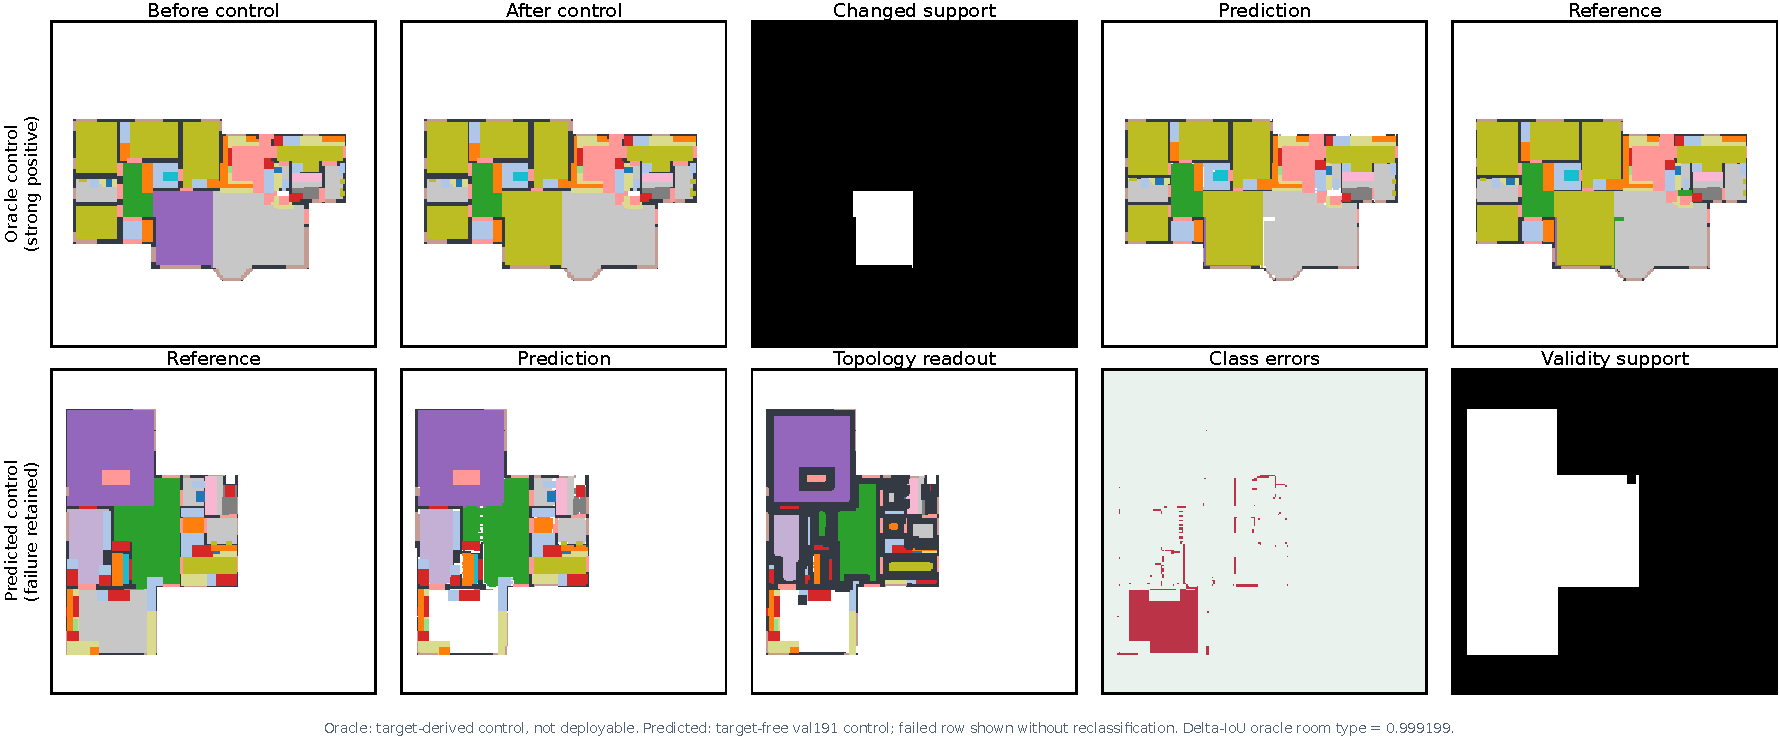
\includegraphics[width=\textwidth]{figures/floorplan_qualitative_cases_v1.pdf}
\caption{Case-level audit. Top: oracle room-type control with before/after
controls, changed support, prediction, and reference. Bottom: a target-free
predicted failure retained without reclassification. Oracle controls are
target-derived; the predicted case is not held out.}
\label{fig:qualitative}
\end{figure*}

\section{Discussion}
The results support a distinction between edit reliability and reference
fidelity. Oracle controls show that the composition and restoration path can
support large local changes while leaving the outside domain exact. Predicted
controls show that the same path preserves the safety contract and produces
geometrically plausible plans even when room identity and graph fidelity are weak.
This is useful for an interactive system because unsafe edits and unsupported
requests can be separated from semantic quality rather than averaged into one
number.

The evidence also exposes the cost of that conservatism. Semantic realization is
uneven, predicted Room macro IoU is low, and the raw watertightness boundary is
visible for multi-component footprints. A system that appears reliable by
preserving the input too aggressively is not sufficient if it fails to realize
the requested operation. We therefore report execution and abstention as safety
outcomes, not as semantic success.

\section{Limitations}
Oracle controls are target-derived and non-deployable. Predicted results come
from an existing validation and development-exposed test exposure, not a fresh
held-out run. Five repeated seeds are not independent plans. Raster2Seq is a
reconstruction wrapper, not a native editing baseline. The editing-aware control
is intentionally weak. Raw and functional watertightness answer different
questions. HouseMind-E is cross-dataset context and the official serialization is
unavailable.

The paper does not claim complete-method SOTA, RPLAN or full-CAD leadership,
deployable free-text control, high predicted room identity, or uniform semantic
success. Move-wall, resize, and free-form global recomposition remain outside the
supported operation set.

\section*{Data and Ethics}
The study uses CubiCasa5K under its research-use terms. It introduces no human
subjects, participant data, or personally identifiable information. The release
excludes datasets, checkpoints, raw tensors, third-party source trees, and
unselected generated outputs. The evidence registry, frozen file identities,
figure case manifest, artifact manifest, and checksums are released with the
manuscript.

\section*{Reproducibility Statement}
Every numerical value in the main tables is bound to
\path{docs/floorplan_submission_source_registry_v2.json} and the frozen
release in \path{configs/floorplan_submission_evidence_freeze_v2.json}.
The provenance and freeze audits are machine-readable. Figure cases are selected
by a recorded deterministic rule and stored in
\path{outputs/reports/floorplan_figure_case_manifest_v1.json}. The artifact
package is anonymous and contains source, tests, selected configurations,
manuscript sources, tables, figures, and selected evidence. It does not contain
datasets or checkpoints.

\section*{LLM Usage Statement}
Large language model assistance was used for code editing, artifact auditing,
LaTeX formatting, and language editing. Numerical claims were checked against the
frozen source registry and generated tables. The reported experiments were not
replaced by model-generated results, and no held-out number, execution receipt,
or venue submission receipt was fabricated. The authors remain responsible for
the final manuscript, data use, and external submission.

{\small
\bibliographystyle{ieeenat_fullname}
\bibliography{references}
}

\end{document}

